% !TEX root = ../SYSprojektrapport.tex
% SKAL STÅ I TOPPEN AF ALLE FILER FOR AT MASTER-filen KOMPILERES 

\section{Case 4: Den centrale batteriparks evne til at kompensere for tab af produktion}
I dette afsnit præsenteres resultater for simuleringen af case 4 iht. beskrivelsen i afsnit \ref{SimCase4}. I alle fire tilstande er spændingsændringen ved Town5 busbar (rød linje) og Transmission central 60kV busbar (Grøn linje) samt frekvensændringen på Transmission central 60kV busbar (Grøn linje), præsenteret på hhv. spændingsgraf og frekvensgraf. Derudover er der lavet opsamling over spænding samt effektoverførelse andre relevante steder i systemet i tabel \ref{fig:C4Overview}. \\ \\

\textbf{Tilstand 1: Alle batterierne er frakoblet.}
\begin{figure}[H]
	\centering
	\begin{minipage}[b]{0.48\textwidth}
		\centering
		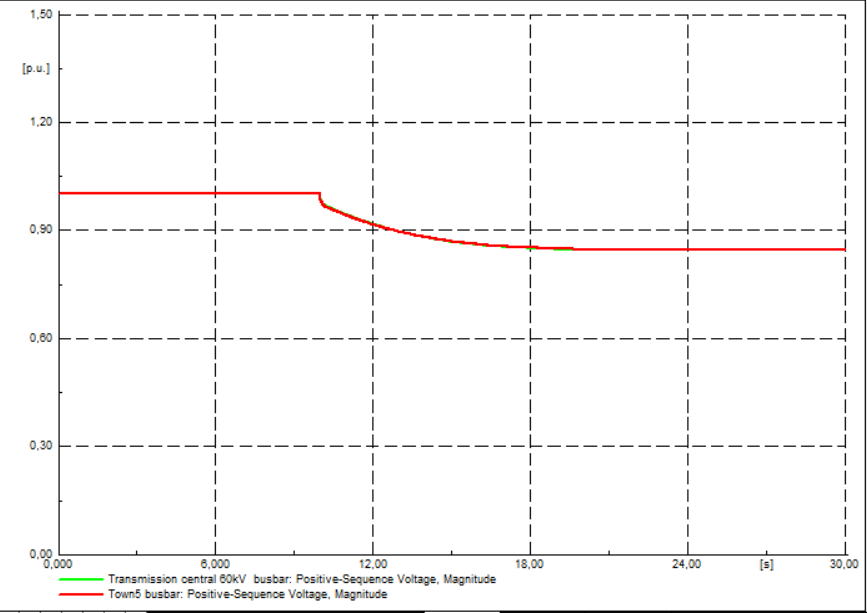
\includegraphics[width=1.00\textwidth]{figurer/LargeDisturbance/Voltage1} % Venstre billede
	\end{minipage}
	\hfill
	\begin{minipage}[b]{0.48\textwidth}
		\centering
		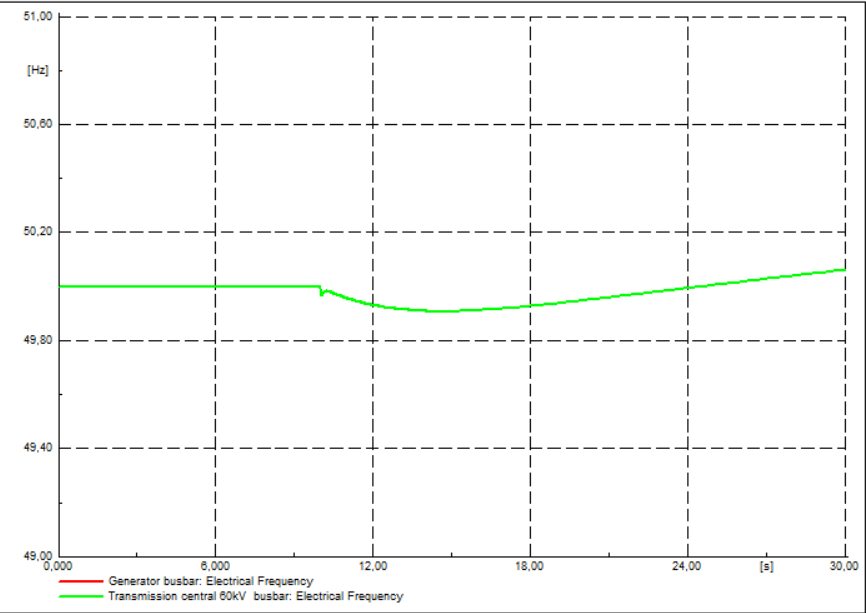
\includegraphics[width=1.00\textwidth]{figurer/LargeDisturbance/Freq1} % Højre billede
	\end{minipage}
	\\ % Figurtekster og labels
	\begin{minipage}[t]{0.48\textwidth}
		\caption{Case 4, Tilstand 1, Spændingsgraf} % Venstre figurtekst og label
		\label{fig:C4T1V}
	\end{minipage}
	\hfill
	\begin{minipage}[t]{0.48\textwidth}
		\caption{Case 4, Tilstand 1, Frekvensgraf} % Højre figurtekst og label
		\label{fig:C4T1F}
	\end{minipage}
\end{figure}

\textbf{Tilstand 2: Batteri central leverer 2,5MW med pf 0,95 lagging.}
\begin{figure}[H]
	\centering
	\begin{minipage}[b]{0.48\textwidth}
		\centering
		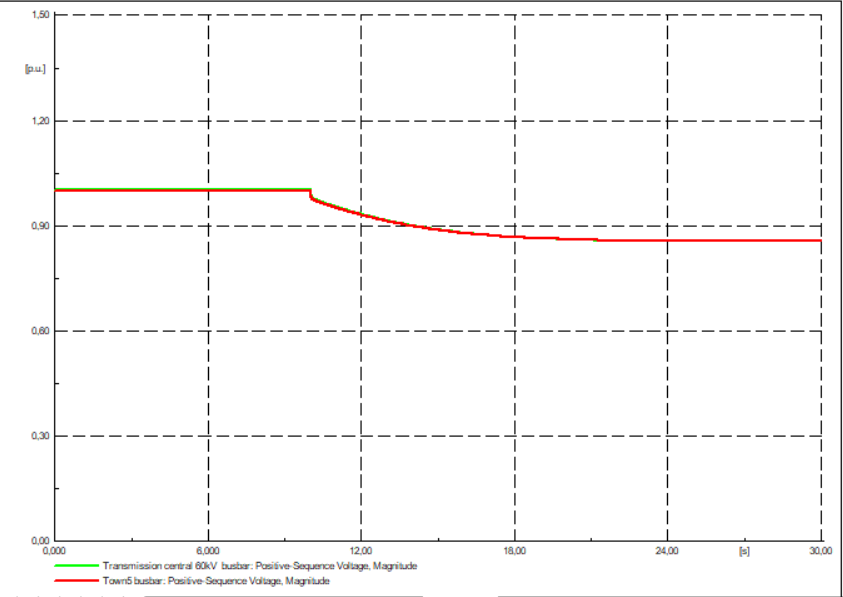
\includegraphics[width=1.00\textwidth]{figurer/LargeDisturbanceBatterypark/Voltage2} % Venstre billede
	\end{minipage}
	\hfill
	\begin{minipage}[b]{0.48\textwidth}
		\centering
		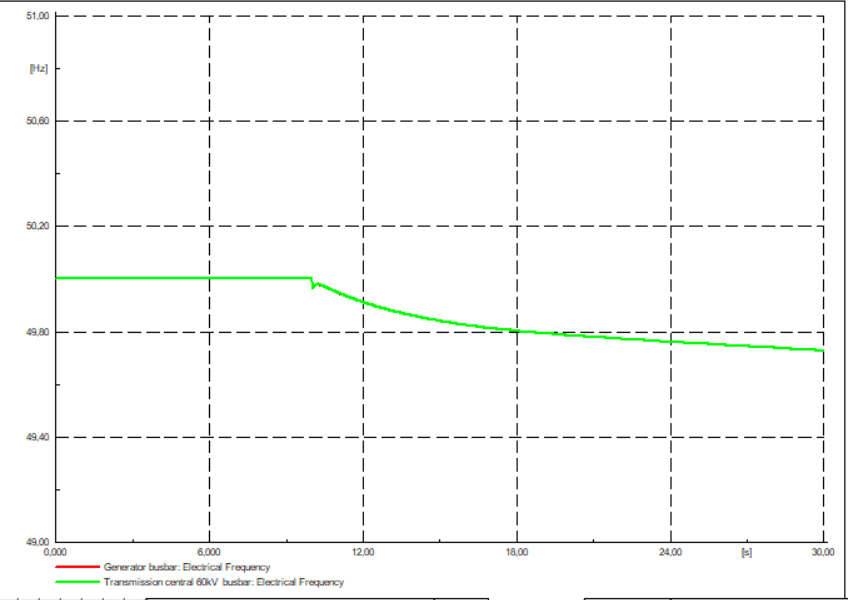
\includegraphics[width=1.00\textwidth]{figurer/LargeDisturbanceBatterypark/Freq2} % Højre billede
	\end{minipage}
	\\ % Figurtekster og labels
	\begin{minipage}[t]{0.48\textwidth}
		\caption{Case 4, Tilstand 2, Spændingsgraf} % Venstre figurtekst og label
		\label{fig:C4T2V}
	\end{minipage}
	\hfill
	\begin{minipage}[t]{0.48\textwidth}
		\caption{Case 4, Tilstand 2, Frekvensgraf} % Højre figurtekst og label
		\label{fig:C4T2F}
	\end{minipage}
\end{figure}

\textbf{Tilstand 3: Batteri central leverer 5MW med pf 0,95 lagging.}
\begin{figure}[H]
	\centering
	\begin{minipage}[b]{0.48\textwidth}
		\centering
		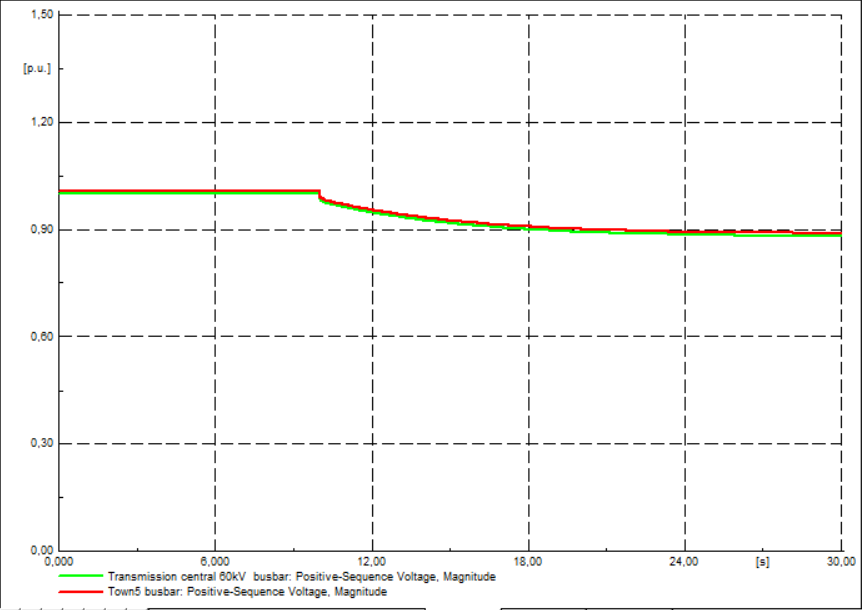
\includegraphics[width=1.00\textwidth]{figurer/LargeDisturbanceBatterypark/Voltage3} % Venstre billede
	\end{minipage}
	\hfill
	\begin{minipage}[b]{0.48\textwidth}
		\centering
		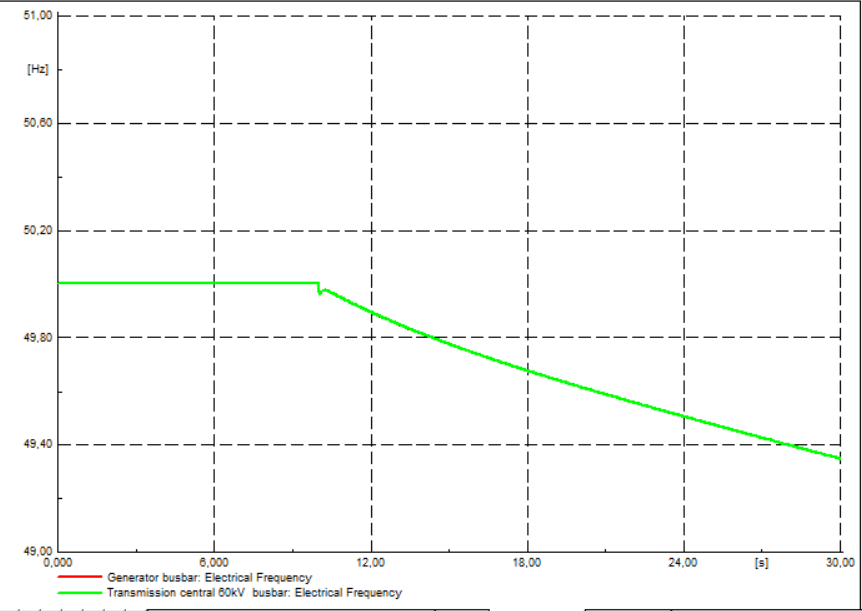
\includegraphics[width=1.00\textwidth]{figurer/LargeDisturbanceBatterypark/Freq3} % Højre billede
	\end{minipage}
	\\ % Figurtekster og labels
	\begin{minipage}[t]{0.48\textwidth}
		\caption{Case 4, Tilstand 3, Spændingsgraf} % Venstre figurtekst og label
		\label{fig:C4T3V}
	\end{minipage}
	\hfill
	\begin{minipage}[t]{0.48\textwidth}
		\caption{Case 4, Tilstand 3, Frekvensgraf} % Højre figurtekst og label
		\label{fig:C4T3F}
	\end{minipage}
\end{figure}

\textbf{Tilstand 4: Batterier leverer 4,41MW med pf 0,95 lagging.}
\begin{figure}[H]
	\centering
	\begin{minipage}[b]{0.48\textwidth}
		\centering
		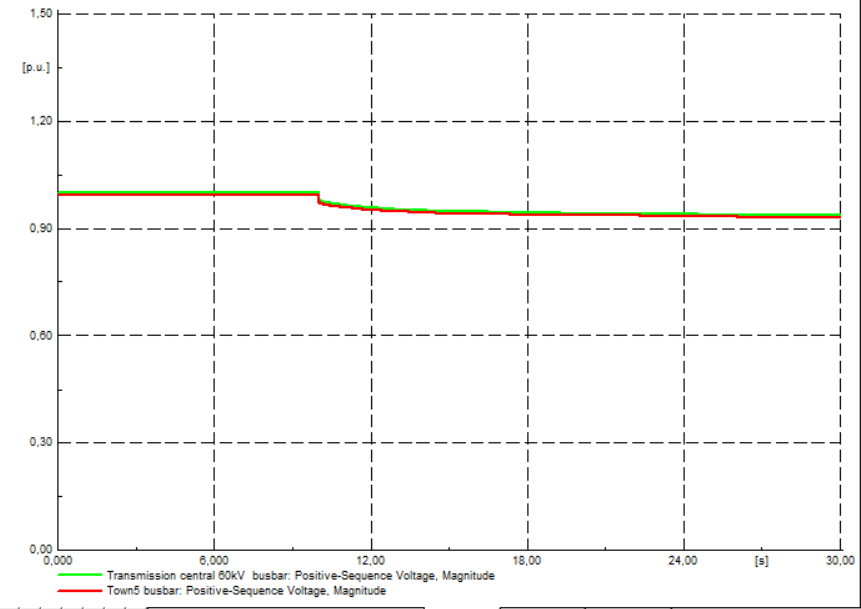
\includegraphics[width=1.00\textwidth]{figurer/LargeDisturbanceBatterypark/Voltage4} % Venstre billede
	\end{minipage}
	\hfill
	\begin{minipage}[b]{0.48\textwidth}
		\centering
		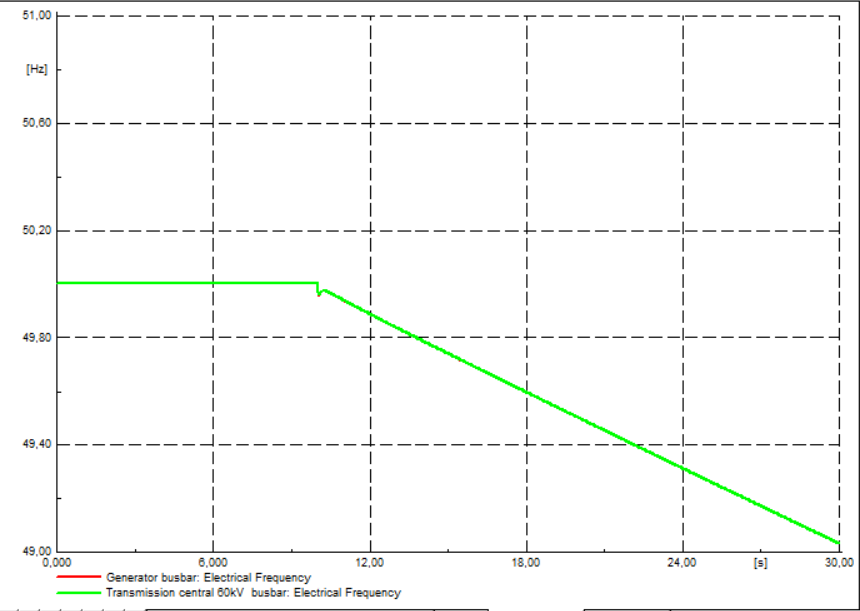
\includegraphics[width=1.00\textwidth]{figurer/LargeDisturbanceBatterypark/Freq4} % Højre billede
	\end{minipage}
	\\ % Figurtekster og labels
	\begin{minipage}[t]{0.48\textwidth}
		\caption{Case 4, Tilstand 4, Spændingsgraf} % Venstre figurtekst og label
		\label{fig:C4T4V}
	\end{minipage}
	\hfill
	\begin{minipage}[t]{0.48\textwidth}
		\caption{Case 4, Tilstand 4, Frekvensgraf} % Højre figurtekst og label
		\label{fig:C4T4F}
	\end{minipage}
\end{figure}

\textbf{Tilstandsoverblik}
\begin{figure}[H] % (alternativt [H])
	\centering
	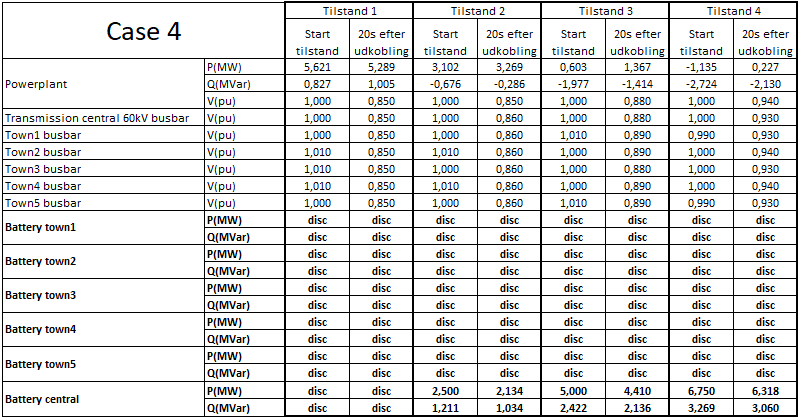
\includegraphics[width=1\textwidth]{figurer/LargeDisturbanceBatterypark/Overview}
	\caption{Overblik for spænding og effektoverførelse i nettet}
	\label{fig:C4Overview}
\end{figure}